\section{Robot}

\begin{frame}
    \frametitle{Le projet SAE Robot}

    
    \begin{figure}[H]
        \centering
        \begin{minipage}{.5\textwidth}
            \centering
            Date de fin de projet : 14 Février 2023
            \\ - \\
            Le cerveau du robot : le microcontrôleur MBED FRDM-KL25Z. Il devra recevoir et envoyer des informations à travers les pins GPIO. 
        \end{minipage}%
        \begin{minipage}{.5\textwidth}
            \centering
            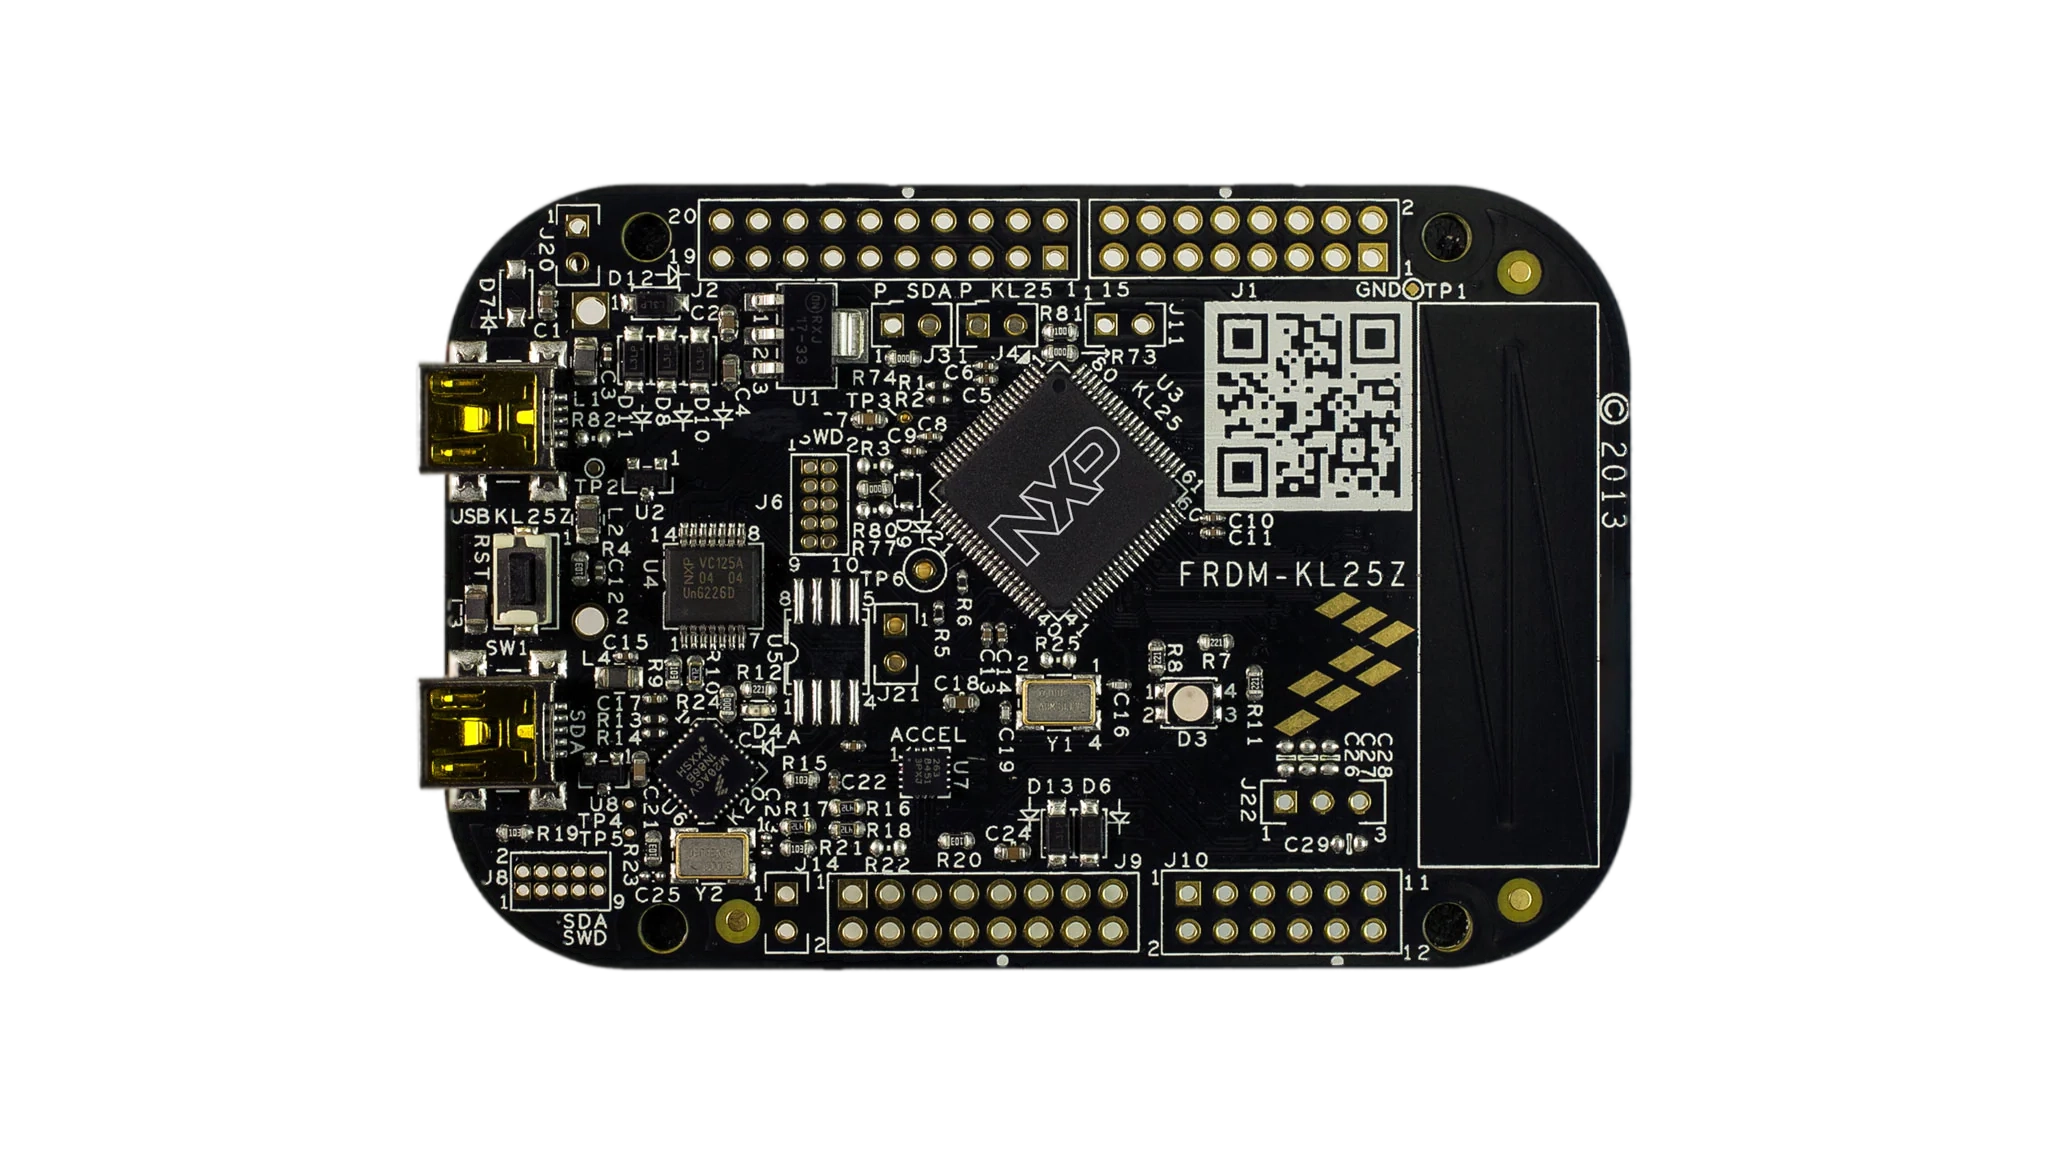
\includegraphics[width=.7\linewidth]{Images/frdmkl25z.png}
            \caption{FRDM-KL25Z}
            \label{fig:µC}
        \end{minipage}%
    \end{figure}
    
\vfill\footer{\hfill\insertframenumber/\inserttotalframenumber}
\end{frame}

 \begin{frame}{Cahier des charges}
    \begin{figure}[H]
        \centering
        \begin{minipage}{.5\textwidth}
            \
            Le robot doit spécifiquement : 
            \begin{itemize}
                \item Évoluer sans aucune aide extérieure.
                \item Suivre le tracé de la piste
                \item Démarrer au retrait d’un câble jack.
                \item S'arrêter lorsque le fin de course s’active en moins de 20 cm.
                \item Fonctionner avec la batterie fournie (12V).
            \end{itemize}
        \end{minipage}%
        \begin{minipage}{.5\textwidth}
            \centering
            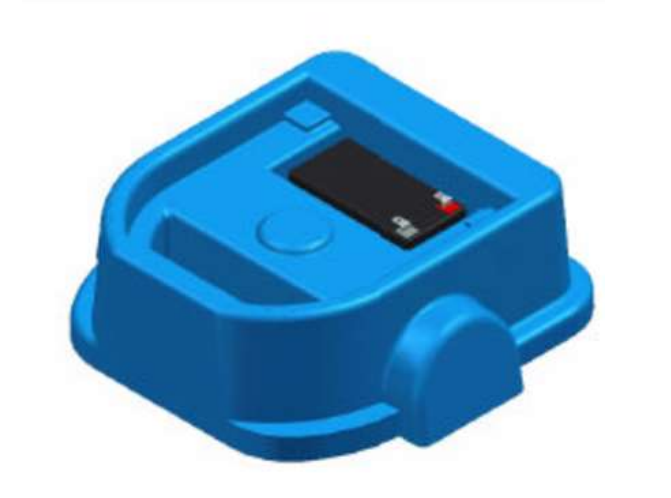
\includegraphics[width=.5\linewidth]{Images/carcasse.png}
            \caption{Châssis fourni}
        \label{fig:carcasse}
        \end{minipage}
    \end{figure}

\vfill\footer{\hfill\insertframenumber/\inserttotalframenumber}
 \end{frame}